\documentclass[conference]{IEEEtran}
\IEEEoverridecommandlockouts

\usepackage{cite}
\usepackage{amsmath,amssymb}
\usepackage{graphicx}
\usepackage{booktabs}
\usepackage{url}
\usepackage[hidelinks]{hyperref}
\usepackage{balance}

\newcommand{\finding}[1]{\textsc{#1}}

\begin{document}

\title{Specified but Not Enacted: Auditing Epistemic\\Control Mechanisms in an Agentic\\Intrusion Triage System}

\author{\IEEEauthorblockN{Author One}
\IEEEauthorblockA{Department\\Institution\\email}
\and
\IEEEauthorblockN{Author Two}
\IEEEauthorblockA{Department\\Institution\\email}
}

\maketitle

\begin{abstract}
Agentic triage systems are increasingly shipped with hand designed epistemic
controls: a hypothesis that cannot be pruned, a gate that boosts doubt, a
decay rule that treats contradicting evidence more harshly than supporting
evidence, and a requirement that a belief persist before it is acted upon.
Such mechanisms are easy to write, easy to describe in a system paper, and
rarely audited. We report an audit of four of them in a working intrusion
triage system, in which a LangGraph reasoning loop sits behind a deep
ensemble sensor trained on UNSW-NB15. The audit is a $2^4$ factorial over the
four mechanisms, crossed with three convergence thresholds and five seeds,
which is 9600 reasoning units against a real language model. Of the four
mechanisms, one works, one works and largely duplicates the first, one is
inert at the resolution five seeds afford, and one is a clamp misdescribed as
a persistence requirement. The sixteen configurations collapse to five
distinct outcomes. We further show that the sensor level of the system's two
level abstention design is never read by the reasoning level: clearing the
abstention flag on every signal in the suite changes the outcome by
$0.000000$. A repair confirms the diagnosis rather than merely asserting it.
Giving a restated hypothesis the identity of its predecessor raises
hypothesis recurrence from $0$ to $0.2045$ and makes the persistence
requirement gate convergence for the first time, at zero additional model
cost. We argue that auditing whether a guardrail is connected should precede
ablating it, since a null effect in an ablation is ambiguous between a
mechanism that does little and a mechanism that is not wired in.
\end{abstract}

\begin{IEEEkeywords}
intrusion detection, LLM agents, abstention, ablation, software auditing,
reproducibility
\end{IEEEkeywords}

\section{Introduction}

\textbf{Hand designed epistemic controls.}
A triage agent that reasons over security alerts must decide not only what is
happening but whether it knows. The common engineering response is to add
explicit machinery for doubt. A hypothesis representing ignorance is made
permanent so that it can always compete. A gate inspects the hypothesis set
and raises doubt when the evidence is thin. Confidence is allowed to fall
faster than it rises. A belief must lead for several consecutive iterations
before the system is permitted to act on it. Each of these is a few dozen
lines of code, each is easy to motivate in prose, and each appears in the
system description as a contribution.

\textbf{The audit question.}
Writing such a mechanism is easy. Establishing that it is connected to
anything is not, and it is almost never attempted. The usual evidence offered
is an ablation: the mechanism is removed, the headline metric moves, and the
mechanism is declared to matter. That argument has a gap at its centre. If
the metric does not move, two very different situations produce the same
table entry. The mechanism may be doing a small amount of real work, or it
may be doing nothing at all because no execution path reaches it. An ablation
alone cannot distinguish them, and the second case is the more alarming of
the two. Thus the usual evidence is weakest exactly where it most needs to
be strong.

\textbf{The system, and what we find.}
We audit four such mechanisms in a working system. The sensor is a deep
ensemble over UNSW-NB15~\cite{moustafa2015} with temperature scaling and a
reject option; the reasoning layer is a LangGraph loop driven by
\texttt{gemini-2.5-flash} over a frozen suite of 40 scenarios containing 66
situations and 963 signals. An information barrier between the two exposes
exactly ten aggregate fields and no raw signal. The four mechanisms are the
non-prunable \textsc{unknown} hypothesis ($U$), the sanity gate ($S$),
asymmetric confidence decay ($A$), and the persistence requirement ($P$).

The result is largely negative, and the negative part is the contribution.
Two of the four mechanisms do nothing that five seeds can resolve. The
sixteen configurations of the factorial collapse to five distinct outcomes,
and $U$ and $S$ determine all five. The effect is concentrated almost
entirely in one evidence regime. The persistence requirement turns out not to
be a persistence requirement at all; it is a clamp that holds the convergence
score just below whatever threshold is configured, and it can never be
satisfied, because the generation step replaces the hypothesis list on every
iteration and no named hypothesis survives long enough to persist. Across 963
multi-iteration analyses and 10{,}068 named hypotheses, not one appears in
two iterations.

Separately, the system is described as abstaining at two levels, once at the
sensor and once in the reasoning loop. The sensor level is not enacted. The
abstention flag is counted into the reasoning snapshot and then read by no
decision, and clearing it on every signal in the suite moves the outcome by
$0.000000$.

\textbf{A repair, not only a diagnosis.}
A diagnosis drawn from code reading and a null effect is correlational, and a
reviewer is entitled to ask whether the mechanism would work if its
precondition held. We therefore repair the precondition. A newly generated
hypothesis inherits the identifier of the prior hypothesis it restates, and
nothing else; descriptions and confidences are left exactly as the model
produced them, so the prompts are unchanged and the experiment costs no
additional model calls. Under the repair, recurrence rises from exactly zero
to $0.2045$, the dominant iteration counter reaches three where it had never
left one, and the persistence requirement gates convergence for the first
time. The mechanism was correctly specified and incorrectly coupled.

\textbf{Contributions.} We offer four. First, an audit method for epistemic
controls that separates \emph{inert} from \emph{disconnected}, and a
five-mechanism verdict table for one real system, see
Section~\ref{sec:findings}. Second, a $2^4$ factorial at 9600 units which
confirms a diagnosis made in advance rather than discovering one after the
fact, see Section~\ref{sec:confirmation}. Third, a prompt-neutral repair
experiment establishing the coupling defect causally, see
Section~\ref{sec:repair}. Fourth, an evaluation hazard of independent
interest, in which a timing defect improves the headline metric by $0.28$
while making the system worse at the only task that requires it to commit,
see Section~\ref{sec:hazards}.

Everything reported here is recomputed from committed machine readable
results by a script that needs no API key and no network; eighteen of
eighteen quoted numbers reproduce on a clean checkout.

\section{Related Work}

\textbf{Machine learning in security, and its evaluation.}
Anomaly detection carries a long survey literature, of which Chandola et
al.~\cite{chandola2009} remains the standard reference. Sommer and
Paxson~\cite{sommer2010} set out why anomaly detection is harder
to evaluate than its literature suggested, and the argument has aged well.
Arp et al.~\cite{arp2022} catalogue ten recurring pitfalls in machine
learning for security and find at least three of them in each of the thirty
papers they examine; sampling bias and inappropriate baselines are the most
common. Pendlebury et al.~\cite{pendlebury2019} show that ignoring temporal
ordering inflates malware classification results to the point of
meaninglessness. Our work sits in this tradition but moves the object of
criticism. Those papers ask whether a reported number is trustworthy. We ask
whether a described mechanism exists in the executed system at all.

\textbf{Technical debt and the specification to implementation gap.}
Sculley et al.~\cite{sculley2015} introduced the vocabulary for this class of
defect, naming boundary erosion, undeclared consumers and configuration debt
among the ways in which machine learning systems accumulate hidden cost. The
defect we report is precisely an undeclared non-consumer: a field is
computed, carried through the system, documented, and read by nobody. Amodei
et al.~\cite{amodei2016} anticipate the general shape of the problem under
the heading of scalable oversight. Neither line of work supplies a
measurement procedure, which is the gap this paper addresses.

\textbf{Testing, and the oracle problem.}
The difficulty of knowing what a correct output looks like is the oracle
problem, surveyed by Barr et al.~\cite{barr2015}, and it is acute for machine
learning systems, surveyed by Zhang et al.~\cite{zhang2022}. Metamorphic
testing~\cite{chen2018metamorphic} addresses it by checking relations between
executions rather than individual outputs. Our ablation is, in this light, a
metamorphic relation of a particular kind: disabling a mechanism that is
genuinely connected must change the output, and we treat a configuration pair
that agrees to four decimal places as a violated relation rather than as a
small effect.

\textbf{Selective prediction and abstention.}
The reject option goes back to Chow~\cite{chow1970}. Modern treatments
include the maximum softmax baseline of Hendrycks and
Gimpel~\cite{hendrycks2017}, the integrated reject option of Geifman and
El-Yaniv~\cite{geifman2019}, and the calibration analysis of Guo et
al.~\cite{guo2017}; our sensor uses a deep ensemble in the style of
Lakshminarayanan et al.~\cite{lakshminarayanan2017} with temperature scaling.
This literature concerns a single classifier that may decline. The system we
audit claims abstention at two levels, and the contribution here is the
finding that the two are not connected.

\textbf{Guardrails for agents, and their evaluation.}
Evaluation of agent guardrails has moved quickly. Das Antar et
al.~\cite{dasantar2025} are closest to this work: they measure the
contribution of individual moderation guardrails and their interactions using
a Bayesian procedure, and they observe that existing evaluations compare
performance with and without the full guardrail stack and so say little about
any single component. Kumar et al.~\cite{nofreelunch2025} report that
guardrails impose measurable utility costs. Recent work on agent safety
reports ablations in which each component is found to be critical.

The distinction we draw is simple and, as far as we can establish, not yet
drawn. All of this work measures \emph{how much} a guardrail contributes,
under the assumption that the guardrail is wired into the execution path.
None of it tests the assumption. We report a system in which that assumption
fails for two of five audited mechanisms, and in which an ordinary ablation
would have recorded the failure as unimportance.

\textbf{LLM agents for triage.}
Multi-agent architectures for alert triage are an active area; CORTEX, for
instance, composes behaviour analysis, evidence gathering and reasoning
agents and reports reduced false positives against single-agent
baselines~\cite{cortex2025}. Such systems are the natural target for the
audit we describe. We make no claim that the system audited here is the strongest
of its kind, and this is deliberate: it is an instrument rather than a
contribution, and the defects we report are of a kind that a stronger system
would be no less likely to carry.

\section{The System Under Audit}

The system has three layers. A sensor consumes UNSW-NB15 flows and emits
signals carrying an anomaly score, a predicted class and an abstention flag;
it is a deep ensemble with temperature scaling and a reject option, and it
abstains on $22.85$\,\% of the signals in the evaluation suite. A situation
store correlates signals by entity into situations. A LangGraph reasoning
loop then runs at most three iterations over each situation, generating
hypotheses with \texttt{gemini-2.5-flash} at temperature $0.2$, evaluating
them against the evidence, and terminating when a convergence score crosses a
threshold whose standing value is $0.8$.

Between the store and the loop sits an information barrier. The context
assembly step exposes exactly ten aggregate fields, among them the evidence
count, the event rate, the burst and quiet indicators, the trend label, the
source diversity and the mean anomaly score. No raw signal, entity
identifier, timestamp or signal identifier crosses it. The barrier is a
deliberate design choice and it has a measurable cost, see
Section~\ref{sec:threats}.

The four audited mechanisms live inside the loop and are individually
removable from the compiled graph rather than merely disabled by a flag.
Figure~\ref{fig:arch} marks where each one acts, and marks two further things
that a conventional block diagram would hide: three adapters that are
written, tested and routed to by nothing, and the abstention path that the
system specifies and does not enact.

\begin{figure*}[t]
\centering
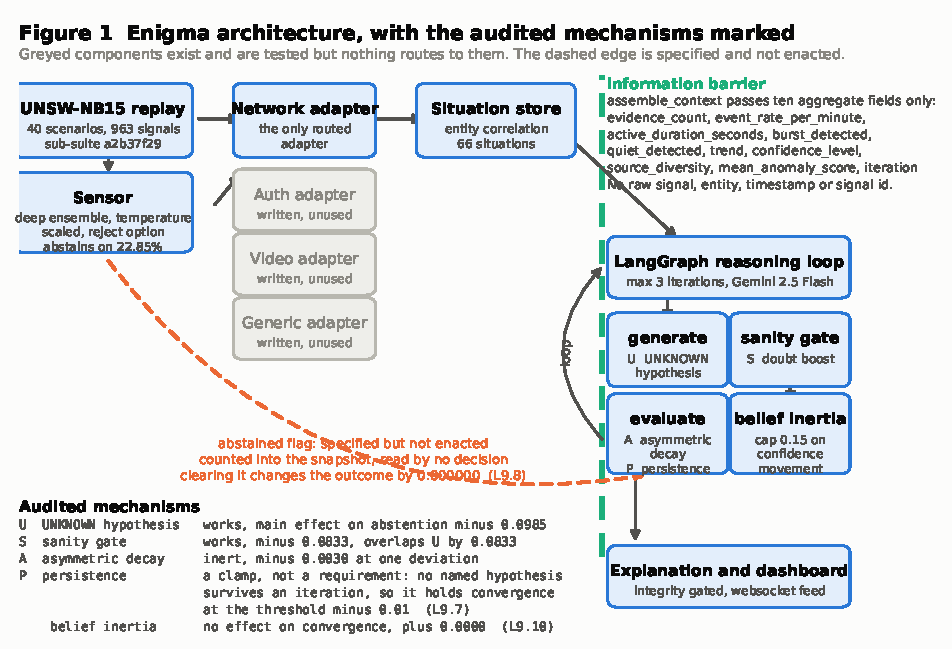
\includegraphics[width=0.92\textwidth]{figures/fig1_architecture.pdf}
\caption{Architecture and data flow, with the audited mechanisms marked.
Solid arrows carry data that is read by a downstream decision. The dashed
green rule is the information barrier: the context assembly step passes the
ten aggregate fields listed beside it and nothing else, so the model never
sees a raw signal, an entity or a timestamp. The three greyed adapters exist
in the source and are exercised by unit tests, and no experiment in this
project routes to them. The dashed orange edge is the sensor abstention path:
the flag is set, carried into the reasoning snapshot, and read by no
decision, so clearing it changes the outcome by $0.000000$, see
Section~\ref{sec:findings}. The four audited mechanisms $U$, $S$, $A$ and
$P$, together with the belief inertia cap, are marked at the graph node at
which each acts.}
\label{fig:arch}
\end{figure*}

\section{Audit Method}
\label{sec:method}

\textbf{A frozen suite with injected ground truth.}
The evaluation suite is generated once, hashed, and never regenerated. The
full suite holds 400 scenarios; the sub-suite used for the factorial holds 40
scenarios, 66 situations and 963 signals, and carries the content hash
\texttt{a2b37f29}. Each scenario is generated in one of four evidence
regimes, which fix what the correct behaviour is. In the \emph{clear} regime
the system should conclude; in the \emph{ambiguous}, \emph{sparse} and
\emph{unknown attack} regimes it should abstain. Ground truth is therefore
injected rather than inferred, which removes the oracle problem for the
abstention metrics, though not for the conclusion metrics, see
Section~\ref{sec:threats}.

\textbf{Metric tiers declared before the run.}
We declared the metric set in the project evidence file before the factorial
executed, and we report it as declared. Four metrics are \emph{live}:
abstention rate, appropriate abstention rate, inappropriate abstention rate,
and premature convergence rate. Each depends only on whether the system
concluded or abstained and on the evidence count at termination, so none
consults a keyword and none depends on narrative identity. Two metrics are
\emph{carried with a caveat}, and two were declared \emph{dead} in advance
because they do not move at the standing threshold. The threshold sweep in
Section~\ref{sec:findings} is the test of whether the dead pair can be
revived at all.

\textbf{Removal, not weakening.}
Each mechanism is ablated by removing its node from the compiled graph, not
by setting a coefficient to zero. Note that this matters for the interpretation; a cell in which a mechanism
is ablated contains no residual trace of it.

\textbf{Content addressed response caching.}
Model responses are cached on a hash of the fully assembled prompt. This
makes a 9600-unit grid affordable, and it makes the grid repeatable. The
realised cache hit rate was $0.9911$, so the grid required only 5851 real
model calls and completed in $2.41$ hours with zero failed units, zero
retries and zero fallback iterations. The caches are scoped per seed, so
replicates remain independent.

\textbf{Design of the factorial.}
The grid is $2^4$ configurations, by three convergence thresholds ($0.30$,
$0.50$, $0.80$), by five seeds, by 40 scenarios: 9600 units. Main effects are
computed per seed as the mean over cells in which a switch is ablated minus
the mean over cells in which it is not, averaged over every combination of
the other three, and the deviation is taken across the five seeds. Two way
interactions are reported as half the difference between the effect of one
switch when a second is ablated and its effect when that second is not.

\section{Audit Findings}
\label{sec:findings}

Table~\ref{tab:verdicts} is the central result. We take the mechanisms in
turn.

\begin{table}[t]
\caption{Verdict on each audited mechanism. Effects are on abstention rate at
the standing threshold $0.80$, ablated minus enabled, five seeds.}
\label{tab:verdicts}
\centering
\small
\begin{tabular}{@{}llr@{}}
\toprule
Mechanism & Verdict & Effect \\
\midrule
\textsc{unknown} hypothesis ($U$) & works & $-0.0985 \pm 0.008$ \\
Sanity gate ($S$) & works, duplicates $U$ & $-0.0833 \pm 0.012$ \\
Asymmetric decay ($A$) & inert & $-0.0030 \pm 0.003$ \\
Persistence ($P$) & a clamp, not a rule & $0.0000 \pm 0.000$ \\
Belief inertia & no effect on convergence & $+0.0000$ \\
Sensor reject option & never read & $+0.000000$ \\
\bottomrule
\end{tabular}
\end{table}

\textbf{\finding{Finding 1. Two mechanisms carry the whole effect.}}
Removing the \textsc{unknown} hypothesis costs $0.0985$ of abstention and
$0.1391$ of appropriate abstention, and buys $0.0970$ of premature
convergence. The effect is twelve standard deviations from zero. The sanity
gate is a genuine second mechanism at roughly five sixths of that size and
with the same sign on every metric. Asymmetric decay moves abstention by
$-0.0030$ against a deviation of $0.003$, which is one deviation from zero on
a metric whose range here is $0.18$; we therefore report it as inert at the
resolution five seeds afford, rather than as absent. The persistence
requirement moves nothing at all: not approximately nothing, but $0.0000$
with deviation $0.0000$ on every live metric.

\textbf{\finding{Finding 2. The sixteen configurations collapse to five.}}
Table~\ref{tab:collapse} gives the structure, which is exact rather than
approximate. The all-on configuration, minus $A$, minus $P$ and minus $AP$
are identical to four decimal places on every metric. The eight
configurations with $U$ disabled are identical to one another: once
\textsc{unknown} is gone, abstention is zero and premature convergence is
$0.6970$ whatever $S$, $A$ and $P$ are set to. Between these extremes, $S$
moves abstention from $0.1818$ to $0.0212$, and $A$ moves it from $0.0212$ to
$0.0091$, but only once $S$ is already off.

\begin{table}[t]
\caption{The sixteen configurations collapse to five distinct outcomes at
threshold $0.80$, five seeds. Rows joined by an equality agree to four
decimal places on all four live metrics.}
\label{tab:collapse}
\centering
\small
\begin{tabular}{@{}lrr@{}}
\toprule
Configuration & Abstention & Premature \\
\midrule
all on $=$ $-A$ $=$ $-P$ $=$ $-AP$ & $0.1818 \pm 0.019$ & $0.5182$ \\
$-S$ $=$ $-SP$ & $0.0212 \pm 0.007$ & $0.6758$ \\
$-SA$ $=$ $-SAP$ & $0.0091 \pm 0.007$ & $0.6879$ \\
all eight with $U$ off & $0.0000$ & $0.6970$ \\
\bottomrule
\end{tabular}
\end{table}

Exactly one two way interaction is resolvable at five seeds. The $U \times S$
term is $+0.0833 \pm 0.0115$, seven times its own spread and as large as the
sanity gate's entire main effect, and it has an interpretation: the two
mechanisms are partly redundant, since both push confidence towards
\textsc{unknown}, so removing both costs less than the sum of removing each.
The $U \times A$ and $S \times A$ terms are each exactly one deviation from
zero, and the three terms involving $P$ are exactly zero because $P$ itself
is exactly zero. We make no interaction claim beyond $U \times S$.

\textbf{\finding{Finding 3. The effect lives in one regime.}}
Broken out by regime, the main effect of $U$ on abstention is $-0.5500 \pm
0.016$ on sparse evidence and $-0.0063 \pm 0.013$ on unknown attacks; for $S$
the corresponding figures are $-0.4500$ and $-0.0063$. On sparse situations
the all-on configuration abstains at $1.0000$ and the minus-$U$ configuration
abstains at $0.0000$, so the mechanism is the difference between always
declining and never declining. On the other three regimes the same switch
moves the rate by between $0.005$ and $0.04$. Figure~\ref{fig:ablation} shows
this directly.

Thus the mechanisms act where evidence is scarce and are close to inert
where the attack is unfamiliar. This is worth stating plainly, because the
unknown attack regime is the one an intrusion triage system would most want
them to work on, and it is the regime on which the two level abstention claim
rests.

\begin{figure*}[t]
\centering
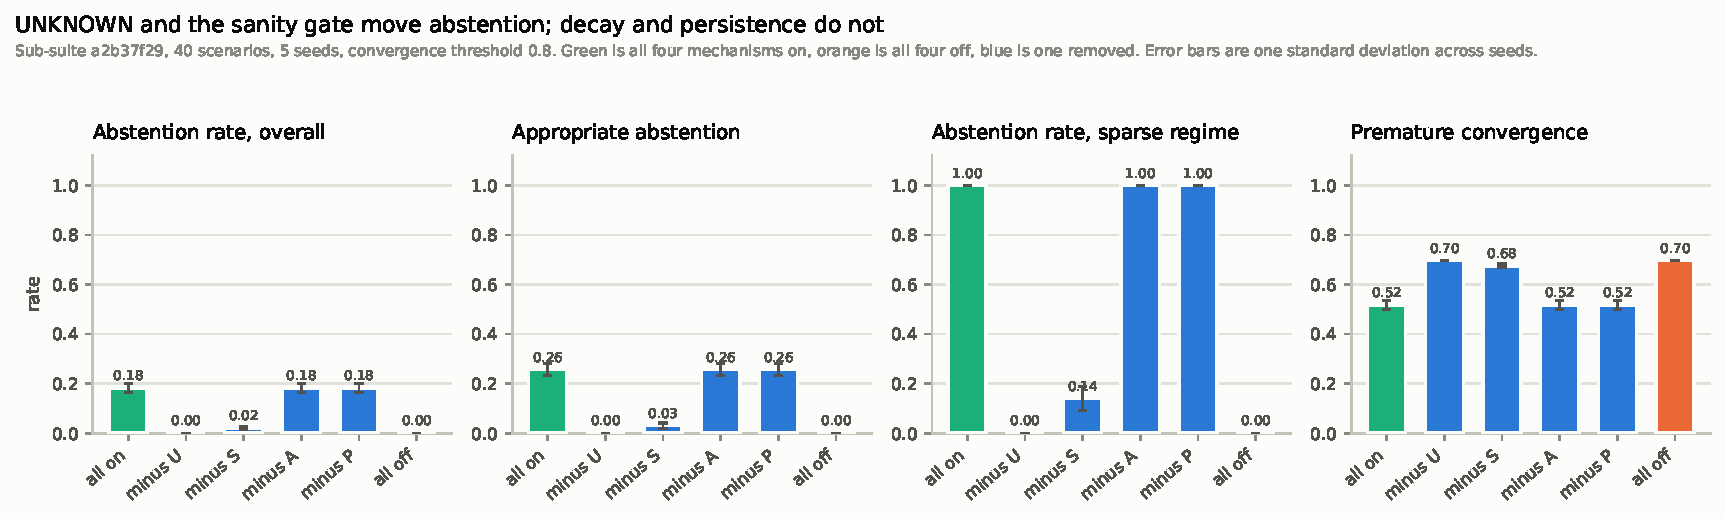
\includegraphics[width=0.96\textwidth]{figures/fig3_ablation_main_effects.pdf}
\caption{Single mechanism removals against the two baselines, sub-suite
\texttt{a2b37f29}, five seeds, threshold $0.80$. Green is the all-on
configuration, orange is all four mechanisms off, blue is one mechanism
removed; error bars are one standard deviation across seeds. The third panel
is not the inappropriate abstention rate, which sits at $0.01$ or below in
all six configurations and would draw six bars on the axis. It is replaced by
the abstention rate on the sparse regime, where the entire effect lives, and
where removing $U$ takes the rate from $1.00$ to $0.00$ while removing $A$ or
$P$ leaves it at $1.00$.}
\label{fig:ablation}
\end{figure*}

\textbf{\finding{Finding 4. Persistence is a clamp, not a requirement.}}
The persistence requirement is implemented by a single line that caps the
convergence score at the threshold minus $0.01$ whenever the dominant
hypothesis has not yet led for the required number of consecutive iterations.
The required number defaults to two, i.e., a belief must lead twice in
succession before it may be acted upon. It is never reached, and the reason is
structural rather than statistical.

The generation step replaces the hypothesis list on every iteration. It
parses a fresh response, builds new hypothesis records with freshly generated
identifiers, and carries forward only the \textsc{unknown} entry, whose
identifier is fixed. The previous iteration's named hypotheses are discarded
rather than updated. Measured over the all-on cell at the standing threshold,
there are 963 analyses of more than one iteration and 10{,}068 named
hypotheses, of which exactly zero appear in more than one iteration; the
dominant iteration counter takes the value $0$ in all 4382 terminated
records; and \textsc{unknown} recurs in all 963. A requirement of two
consecutive dominant iterations is thus unsatisfiable by construction.

The threshold sweep confirms the consequence. With persistence enabled the
convergence fraction is $0.0000$ at every threshold, and the maximum
convergence score reached is exactly the threshold minus $0.01$: $0.2900$ at
$0.30$ and $0.4900$ at $0.50$. That is not a property of the confidence
dynamics; it is the literal value of the clamp. With persistence ablated the
convergence fraction at threshold $0.30$ is $0.5561$. Hence lowering the threshold alone revives
nothing, which answers the question the dead metric pair was declared to
test.

We isolated the clamp from belief inertia, the other mechanism that could
plausibly hold convergence down, by crossing the two at threshold $0.30$ with
everything else enabled. Removing persistence moves the convergence fraction
by $+0.3057$; removing inertia moves it by $+0.0000$, and leaves the maximum
convergence at exactly $0.2900$. Inertia is not entirely idle, but its effect
appears only once persistence has been removed, and it concerns how
convergence is reached rather than whether: with persistence off, lifting the
inertia cap raises the single iteration conclusion rate from $0.0897$ to
$0.1437$ and lowers mean iterations from $2.6640$ to $2.6000$. That is a
mechanism behaving as designed, masked completely by one that is not.

Figure~\ref{fig:trajectory} shows the mechanism directly, and it is not the
figure we set out to draw.

\begin{figure}[t]
\centering
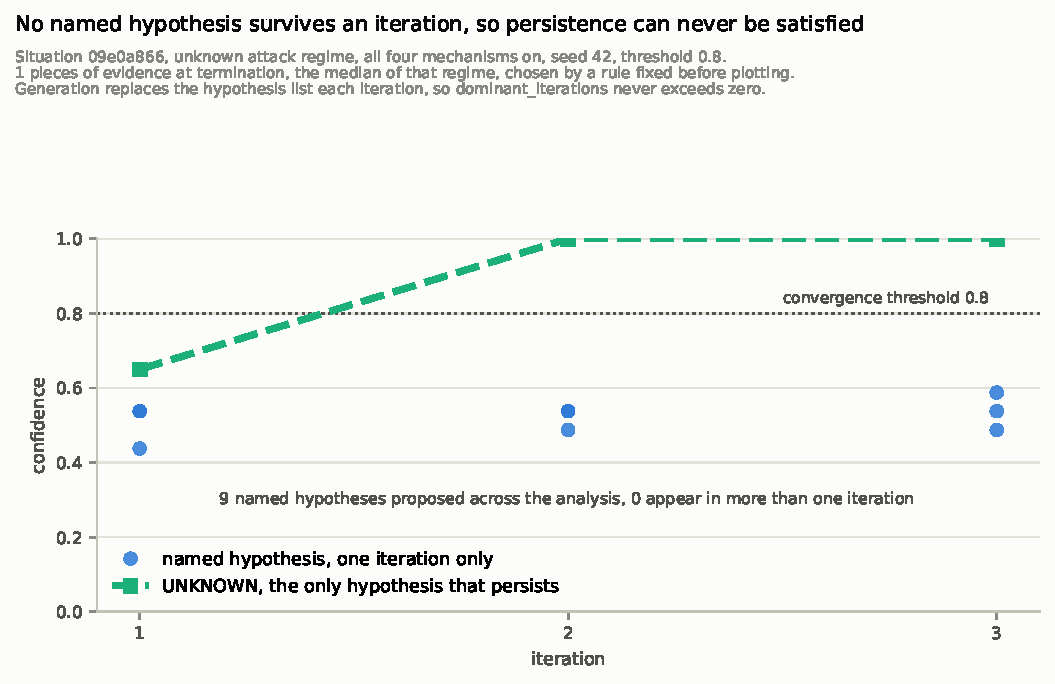
\includegraphics[width=0.95\columnwidth]{figures/fig6_belief_trajectory.pdf}
\caption{Belief trajectory for one situation, chosen by a rule fixed before
any trajectory was plotted: among unknown attack situations of the all-on
cell at seed 42, the one whose evidence count at termination is the median of
its regime, ties broken by the smallest identifier. The dashed green line is
\textsc{unknown}, which climbs from $0.65$ to $0.99$ and is the only
hypothesis that persists. The blue markers are named hypotheses; they are
markers and not lines because none of the nine proposed during the analysis
appears in a second iteration. The dotted rule is the active convergence
threshold. The absent trajectories are the finding: with no named hypothesis
surviving an iteration, the dominant iteration counter cannot accumulate and
the persistence requirement cannot be satisfied.}
\label{fig:trajectory}
\end{figure}

\textbf{\finding{Finding 5. The second abstention level is never read.}}
The system is described as abstaining twice, once at the sensor and once in
the reasoning loop. We tested the sensor level directly on the unknown attack
regime with a four cell design, crossing the sensor reject option with the
epistemic controls at five seeds. The sensor level is disabled by clearing
the abstention flag on every signal before ingestion, which is the strongest
intervention available.

The two sensor rows are identical. The effect of clearing every abstention
flag is $+0.000000$ with the epistemic controls on, and $+0.000000$ with them
off. The levels are neither complementary nor redundant; the second never
receives the first. Note that the flag is counted into the reasoning snapshot as an abstained
evidence count and an abstained fraction, and is then read by nothing: it does not filter evidence, it does not enter the mean anomaly
score, the source diversity or the confidence level, and it is absent from
the ten fields the information barrier exposes, so the model never sees it.
The suite carries an abstained fraction of $0.2285$ overall and $0.5467$ on
the unknown attack regime, and all of it is inert.

The honest statement is that the two level abstention design is not
implemented, and that this experiment is what establishes it, rather than a
reading of the source. The four cell design was run as specified, and its
sensor axis has no effect because there is no path through which it could
act.

\section{Ablation as Confirmation}
\label{sec:confirmation}

The order in which the evidence was obtained matters, and we state it
explicitly, because it is what separates a prediction from a story told
afterwards.

The persistence clamp was identified during a mock rehearsal of the grid,
before any real model call was spent on the factorial. The rehearsal commit
records that every configuration with persistence enabled sat at a
convergence score of $0.2900$, which is the threshold minus $0.01$, and names
the clamp as the cause. The factorial then confirmed it at 9600 units against
a real model, and the isolation experiment confirmed it again against the one
competing explanation.

This ordering is the methodological point of the paper. Had the grid been run
first, the result would have been a table in which $A$ and $P$ have null
effects, and the natural reading of such a table is that the two mechanisms
are unimportant. The correct reading for $P$ is that it is not wired to
anything it could affect, and for the sensor reject option that no path
exists at all. Those are different defects with different remedies, and an
ablation cannot tell them apart. We therefore propose a simple discipline:
before ablating a mechanism, establish by inspection or by instrumentation
that a path exists from the mechanism to the metric, and report that check
alongside the ablation.

\section{The Repair Experiment}
\label{sec:repair}

A diagnosis from code reading plus a null effect is correlational. The direct
test is to supply the missing precondition and to see whether the mechanism
then works.

\textbf{Design, fixed before running.}
A newly generated hypothesis inherits the identifier and the dominant
iteration counter of the prior hypothesis it restates, and nothing else. The
description and the confidence remain exactly as the model produced them. The
prompt prints only descriptions and confidences, so every prompt a repaired
run issues is byte identical to one the unrepaired run already issued, and
early termination can only shorten an analysis. The repair is thus prompt
neutral by construction, which the budget gate then confirmed: across
42{,}863 cache lookups the repaired grid produced zero cache misses and cost
nothing.

\textbf{The matching rule.}
Two hypotheses are matched by normalising to lowercase alphanumeric words and
comparing with a sequence matcher, accepting at or above $0.70$, assigning
greedily and one to one in descending similarity. The threshold was
calibrated against the baseline logs before the repair was run. We emphasise
that this is identity matching \emph{within} one analysis, between
consecutive iterations of the same loop, which is a far easier problem than
matching free text to a ground truth catalogue; the two texts are produced
seconds apart by the same model about the same situation. The calibration
bears this out: in the baseline logs, 917 consecutive iteration pairs are
byte identical text that nonetheless received a fresh identifier.

Thirty matched chains were sampled and read by hand against a bar of 24. All
thirty are the same hypothesis restated. One is borderline and is recorded as
such, the subject being unchanged while the severity wording flips; counting
it against still leaves 29 of 30.

\textbf{Result.} Table~\ref{tab:repair} gives the comparison. The baseline is
the all-on cell of the factorial at the same threshold and seed, and is not
re-run.

\begin{table}[t]
\caption{Repair against baseline, five seeds, 40 scenarios. Recurrence is the
fraction of named hypotheses appearing in more than one iteration, and
$d_{\max}$ is the largest dominant iteration counter observed.}
\label{tab:repair}
\centering
\small
\begin{tabular}{@{}llrrrr@{}}
\toprule
Thr. & Arm & Recur. & $d_{\max}$ & Conv. & Max conv. \\
\midrule
$0.30$ & baseline & $0.0000$ & $1$ & $0.0000$ & $0.2900$ \\
$0.30$ & repair   & $0.2045$ & $3$ & $0.1551$ & $0.4530$ \\
$0.50$ & baseline & $0.0000$ & $1$ & $0.0000$ & $0.4620$ \\
$0.50$ & repair   & $0.2029$ & $3$ & $0.0000$ & $0.4620$ \\
$0.80$ & baseline & $0.0000$ & $1$ & $0.0000$ & $0.4620$ \\
$0.80$ & repair   & $0.2029$ & $3$ & $0.0000$ & $0.4620$ \\
\bottomrule
\end{tabular}
\end{table}

Identity is restored: recurrence rises from exactly zero to $0.2045$, and the
dominant iteration counter reaches three where it had never left one. The
distribution of that counter at threshold $0.30$ moves from
$\{0{:}300,\,1{:}663\}$ in the baseline to
$\{0{:}300,\,1{:}328,\,2{:}250,\,3{:}85\}$ under the repair, so 335 analyses
now satisfy a requirement that no analysis had ever satisfied.

Persistence then gates convergence. At threshold $0.30$ the convergence
fraction rises from $0.0000$ to $0.1551$, mean iterations falls below three
for the first time, and the maximum convergence score rises from $0.2900$,
which is exactly the clamp, to $0.4530$, which is the dynamics. The verdict
is that the mechanism was correctly specified and incorrectly coupled.

\textbf{Two limits, and a second ceiling.}
At thresholds $0.50$ and $0.80$ the convergence fraction stays at zero, and
this is not the clamp. The maximum convergence under the repair is $0.4620$
at both, below either threshold, so something else binds. Inspection of the
source identifies two contributing causes. First, the convergence score is
not the confidence of the dominant hypothesis but a spread statistic, of the
form $\min(2\sigma + \mu/2,\, 1)$, where $\sigma$ is the gap between the
largest and the mean confidence and $\mu$ is the margin over \textsc{unknown},
further multiplied by penalties when the distribution is flat. Second, a
newly generated hypothesis has its confidence constrained to the interval
$[0.1, 0.5]$ at birth. Both bound the achievable score well below the
standing threshold. We report this as a second structural ceiling,
established by code inspection and consistent with the measurement, and we
did not run the experiment that would separate the two causes.

The second limit is that recurrence reaches $0.2045$ and not $1.0$. Four
named hypotheses in five are still genuinely new at each iteration, so the
repair helps the fifth. Whether that is a ceiling of the matching rule or of
the model's generation behaviour is not established here.

\section{An Evaluation Hazard}
\label{sec:hazards}

The audit turned up a second result of independent interest, concerning the
way a timing defect interacts with an abstention metric.

The system reasons over archived events, and a staleness check decides
whether a situation is quiet. If that check evaluates the age of the evidence
in host time while the events themselves carry archival timestamps, the two
clocks are conflated and every situation appears old. We parameterised the
defect and ran three clock modes at five seeds.

Under conflation, the quiet fraction is $1.0000$ in all five seeds: every
situation is marked quiet. Trend detection collapses with it, and the
conflated mode emits only two distinct trend labels against three for the
correct mode, the stable label never being emitted across 14{,}445
iterations.

The hazard is what then happens to the headline metric, see
Figure~\ref{fig:clock}. Under conflation the rate of correct conclusions
rises from $0.22$ to $0.50$. A reader presented with that number alone would
conclude that the defective configuration is the better one.

It is an abstention artefact. Marking every situation quiet drives the
abstention rate from $0.1818$ to $0.5273$, and since three of the four
regimes score an abstention as correct, abstaining more often scores better.
On the single regime that requires the system to commit, the defect makes it
worse, taking the clear regime rate from $0.130$ to $0.080$. The hazard
generalises beyond this system: any replay based evaluation that scores
abstention as correct in most regimes, and that evaluates staleness against
wall clock time rather than against event time, will reward the defect; the
hazard is a property of the scoring rule, not of this corpus. We note also that the hazard has a
threshold rather than a gradient; a quiet fraction of $0.21$ changes nothing,
and a quiet fraction of $1.00$ changes everything.

\begin{figure}[t]
\centering
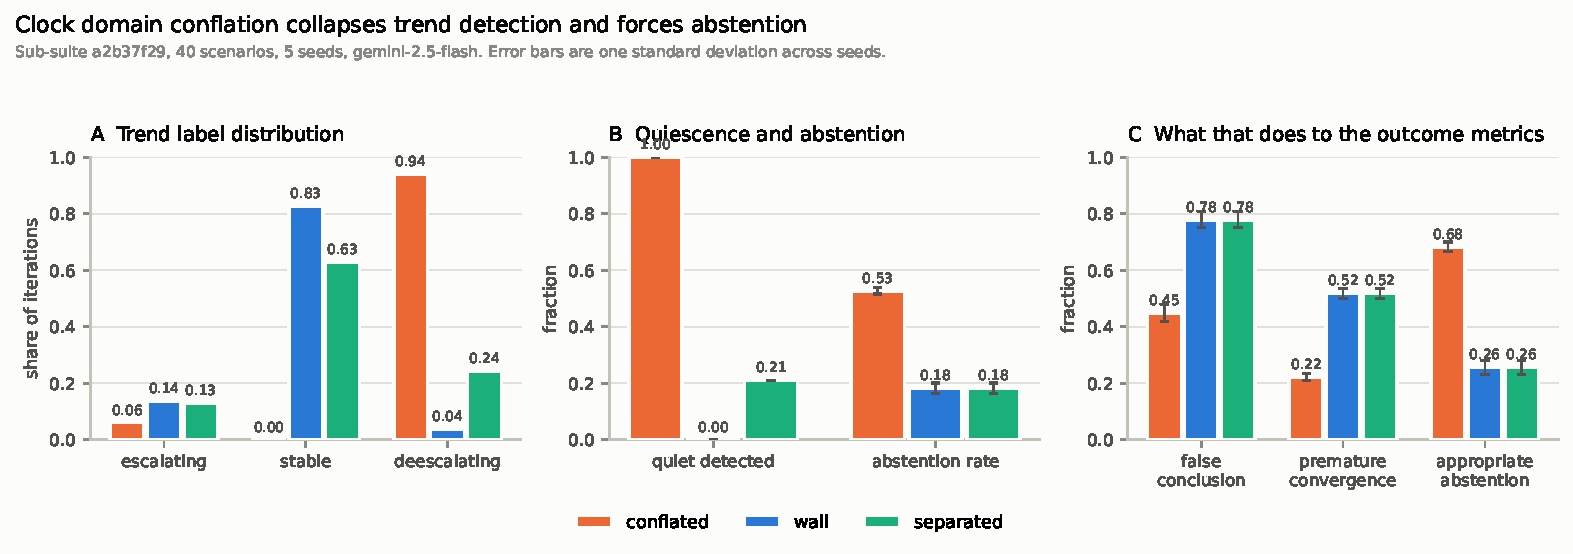
\includegraphics[width=0.95\columnwidth]{figures/fig2_clock_collapse.pdf}
\caption{Collapse of the temporal layer under clock conflation, five seeds.
The three groups are the conflated mode, in which staleness is evaluated in
host time while events carry archival timestamps, the wall clock mode, and
the correctly separated mode. Under conflation the quiet fraction is
$1.0000$ in every seed and the stable trend label is never emitted. The
abstention rate rises from $0.1818$ to $0.5273$, which raises the rate of
correct conclusions from $0.22$ to $0.50$ even though the clear regime, the
only one in which the system must commit, falls from $0.130$ to $0.080$.}
\label{fig:clock}
\end{figure}

\section{Threats to Validity}
\label{sec:threats}

\textbf{Scale and synthesis.} The evaluation is synthetic throughout. There
is no deployment and no operator study. The sub-suite holds 40 scenarios and
66 situations, so a per regime cell carries about 16 situations and a
binomial interval of roughly $\pm 0.245$ at 95\,\%. Five seeds support the
main effects and the single interaction we claim; we claim no significance
test.

\textbf{Narrative identity is not recoverable.} The ten fields the
information barrier exposes separate the four evidence regimes with a lift of
$0.288$ over the base rate, and carry no information about which narrative a
scenario is about, at a lift of $-0.105$. Two of the six narrative categories
share an identical detector signature and are indistinguishable by
construction. Hence any metric that checks whether the system named the right attack is
measuring vocabulary overlap, and we exclude the
conclusion metrics from every claim in this paper. They are reported in the
supporting material with the caveat attached.

\textbf{The instrument.} The sensor is a component rather than a
contribution, and is characterised only to the extent the audit requires. The
multi source condition in the suite is constructed rather than observed. The
confidence weighting coefficients inside the evaluation step were never
swept, so we cannot exclude the possibility that some of the inertia of the
system is an artefact of their values.

\textbf{Non-determinism.} The language model is non-deterministic. Caches are
scoped per seed so that replicates remain independent, and the grid recorded
zero fallback iterations, so no result here rests on a degraded path.

\textbf{Generality.} Every finding is from one system. The conflation hazard
in particular is demonstrated on one corpus that happens to be uniformly
stale, and the threshold behaviour rests on two observations rather than on a
curve. What we claim to generalise is the method, and the ambiguity it
resolves, rather than the specific verdicts.

\section{Reproducibility}

A single script at the project root regenerates every figure in this paper
and recomputes every number it quotes, from committed machine readable
results, with no API key and no network. On a clean checkout it reports five
stages passed, zero failed, and eighteen of eighteen quoted numbers
reproducing within $5 \times 10^{-4}$. Running it on a clean checkout found
two real defects in our own artefacts, which is the only reason to run such a
script rather than merely to ship it.

Across the project, $91.2$\,\% of 130{,}436 model calls were served from the
content addressed cache rather than paid for twice. The repair experiment of
Section~\ref{sec:repair} was served entirely from cache and cost nothing,
which is a direct consequence of its prompt neutrality rather than a
convenience.

\section{Conclusion}

Of four hand designed epistemic controls in a working intrusion triage agent,
one works, one works and largely duplicates the first, one is inert at the
resolution five seeds afford, and one is a clamp misdescribed as a
persistence requirement. A fifth mechanism, the sensor's reject option, is
specified and not enacted: clearing it on every signal in the suite changes
the outcome by $0.000000$. A prompt-neutral repair confirms the persistence
diagnosis causally, raising recurrence from zero to $0.2045$ and making the
mechanism gate convergence for the first time.

The general lesson concerns the order of operations. A null effect in an
ablation is ambiguous between a mechanism that does little and a mechanism
that is not connected, and the two call for entirely different responses. We
therefore suggest that establishing the existence of a path from mechanism to
metric should precede measuring the size of the effect along it. Guardrails
are easy to write and hard to verify, and in the system examined here three
of five did not survive being measured.

\balance
\bibliographystyle{IEEEtran}
\bibliography{refs}

\end{document}
